
\section{Sensitivity analyses}
\subsection{Sensitivity analysis using alternative base mixing matrices}
We ran an alternative sensitivity analysis using the mixing matrices from Prem et al. 2020, which is currently available as a pre-print, rather than those from the 2017 publication. The results of this analysis were similar to that of the baseline analysis and are presented in Figure \ref{fig:prem_sensitivity_outputs}, Figure \ref{fig:prem_sensitivity_key_params} and Figure \ref{fig:prem_sensitivity_epi_params}.

\begin{figure}[ht]
    \resizebox{1\textwidth}{!}{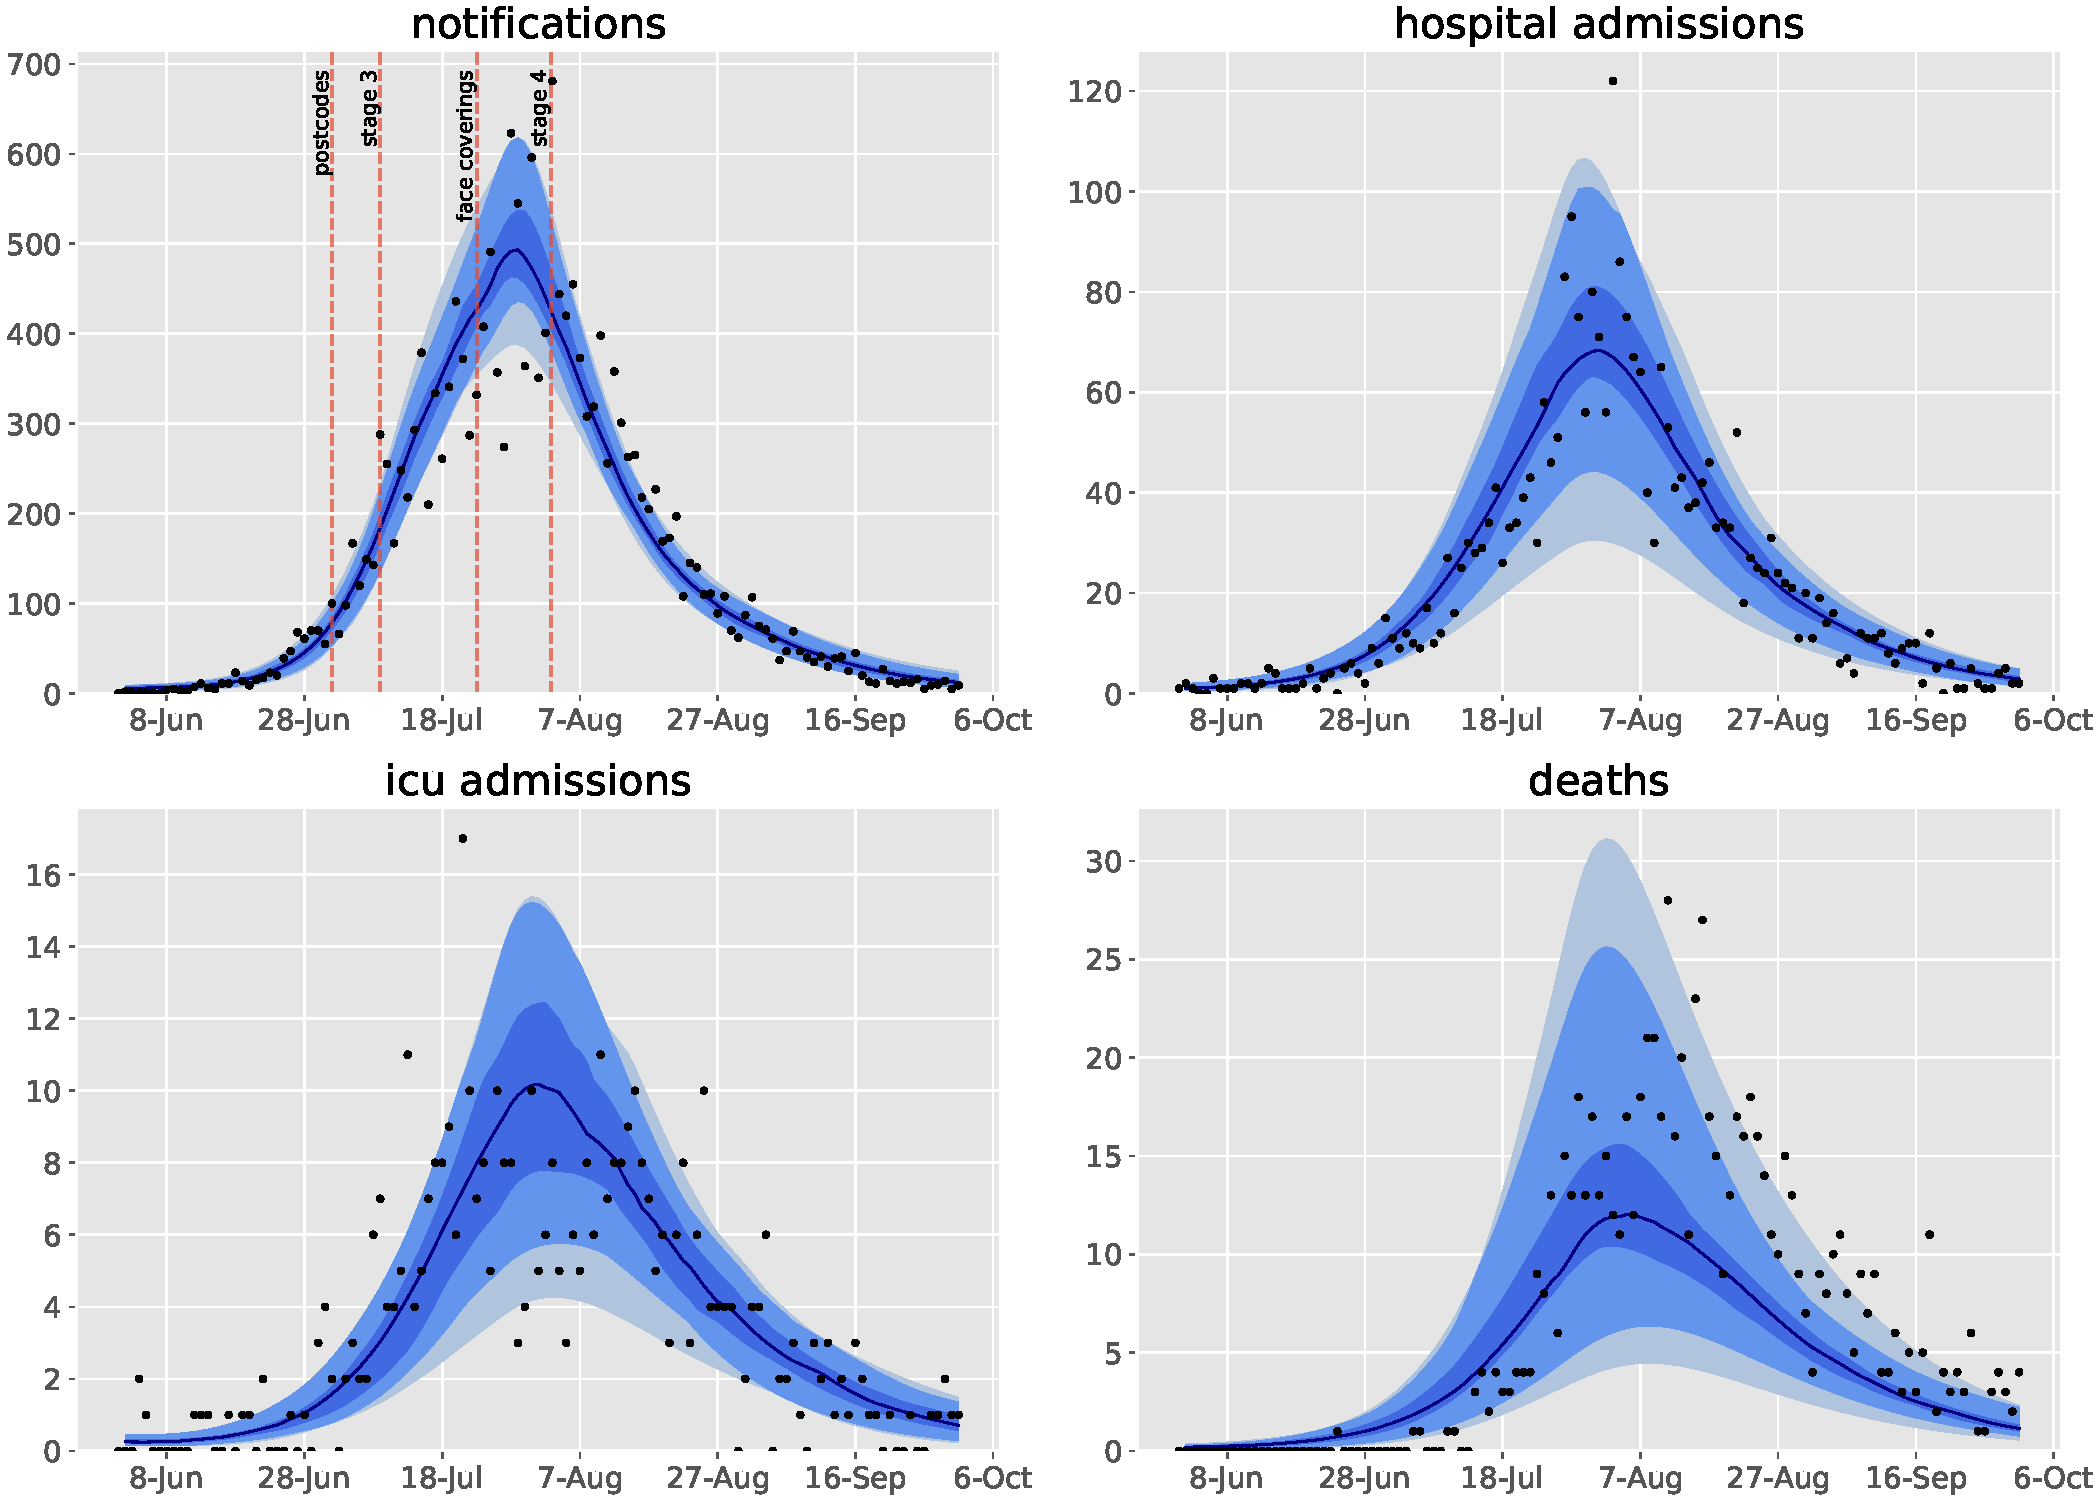
\includegraphics[scale=1]{../covid_19/projects/victoria/prem_sensitivity/multi_output.png}}
    \caption{\textbf{Model fit to statewide indicators using matrices from Prem 2020.}}
    \label{fig:prem_sensitivity_outputs}
\end{figure}

\begin{figure}[ht]
    \resizebox{1\textwidth}{!}{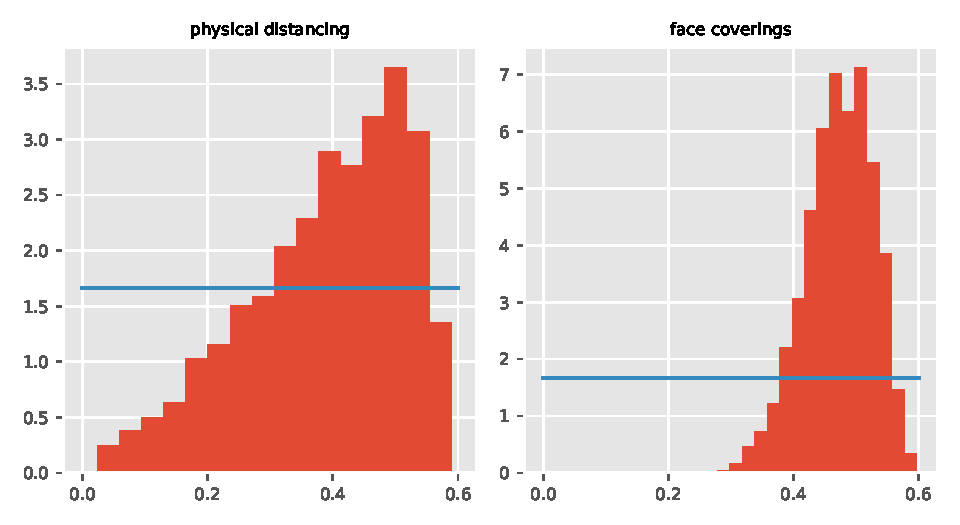
\includegraphics[scale=1]{../covid_19/projects/victoria/prem_sensitivity/key_posteriors.png}}
    \caption{\textbf{Posterior distributions of key model parameters using matrices from Prem 2020.}}
    \label{fig:prem_sensitivity_key_params}
\end{figure}

\begin{figure}[ht]
    \resizebox{1\textwidth}{!}{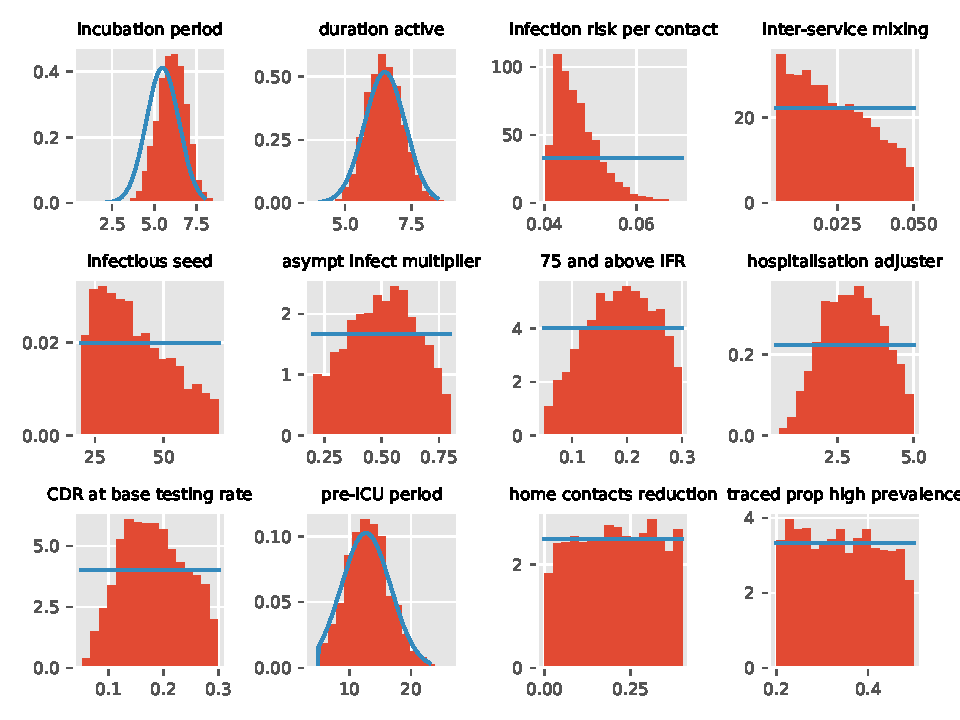
\includegraphics[scale=1]{../covid_19/projects/victoria/prem_sensitivity/epi_posteriors.png}}
    \caption{\textbf{Posterior distributions of epidemiological parameters using matrices from Prem 2020.}}
    \label{fig:prem_sensitivity_epi_params}
\end{figure}

\subsection{Sensitivity analysis with Google residential mobility used to scale home location contribution to mixing matrices}
We ran an alternative analysis, in which the home location contribution to the dynamic mixing matrices scaled with Google residential mobility data. This replaced the baseline assumption that the rates of home location contacts remained fixed throughout the simulations. The results of this analysis were similar to that of the baseline analysis and are presented in Figure \ref{fig:residential_sensitivity_outputs}, Figure \ref{fig:residential_sensitivity_key_params} and Figure \ref{fig:residential_sensitivity_epi_params}.

\begin{figure}[ht]
    \resizebox{1\textwidth}{!}{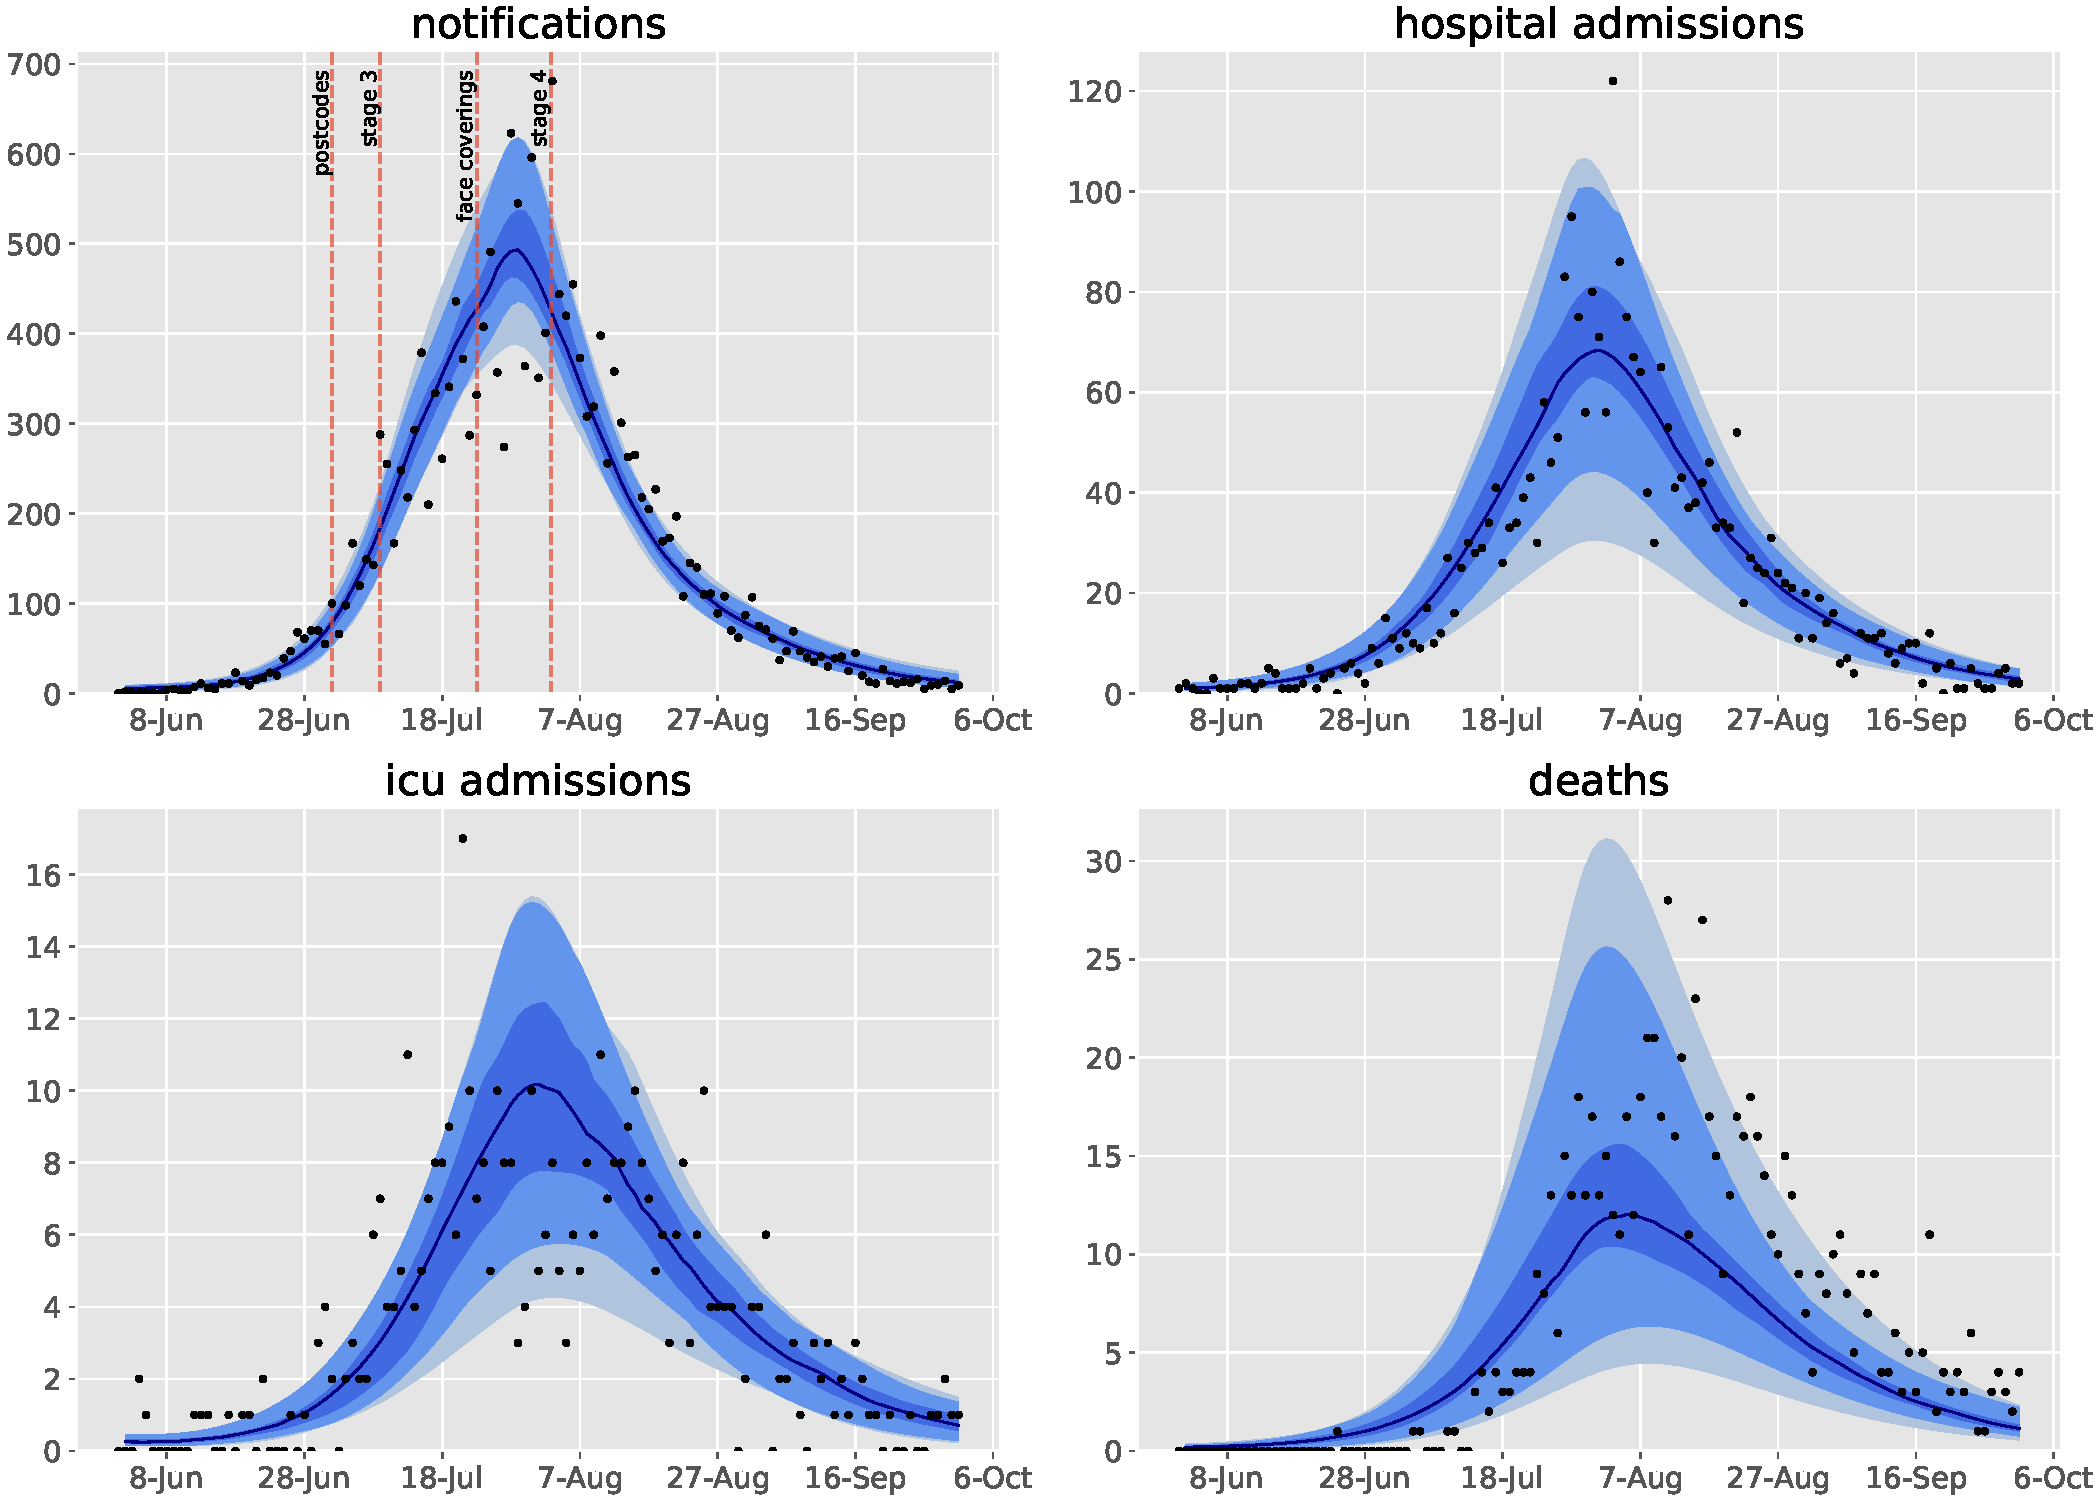
\includegraphics[scale=1]{../covid_19/projects/victoria/prem_sensitivity/multi_output.png}}
    \caption{\textbf{Model fit to statewide indicators mapping Google residential mobility to home locations of mixing matrices.}}
    \label{fig:residential_sensitivity_outputs}
\end{figure}

\begin{figure}[ht]
    \resizebox{1\textwidth}{!}{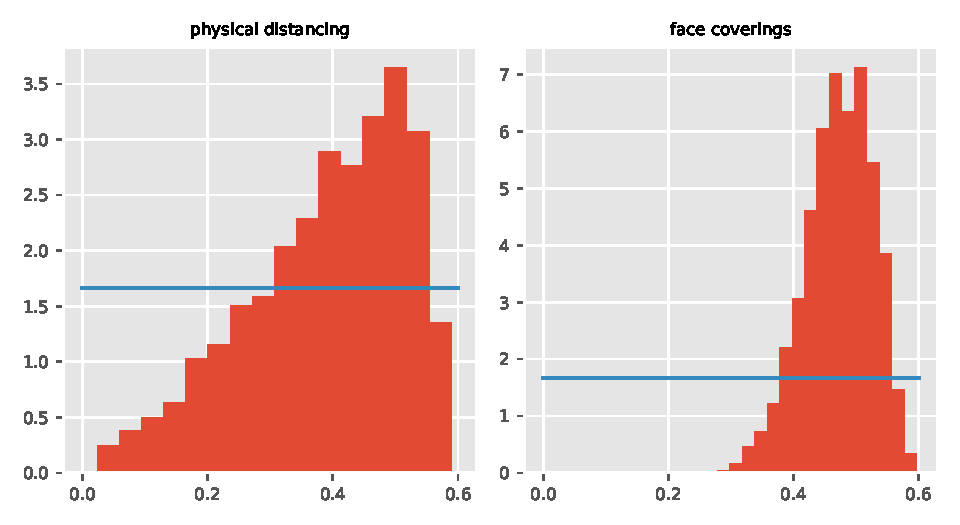
\includegraphics[scale=1]{../covid_19/projects/victoria/prem_sensitivity/key_posteriors.png}}
    \caption{\textbf{Posterior distributions of key model parameters mapping Google residential mobility to home locations of mixing matrices.}}
    \label{fig:residential_sensitivity_key_params}
\end{figure}

\begin{figure}[ht]
    \resizebox{1\textwidth}{!}{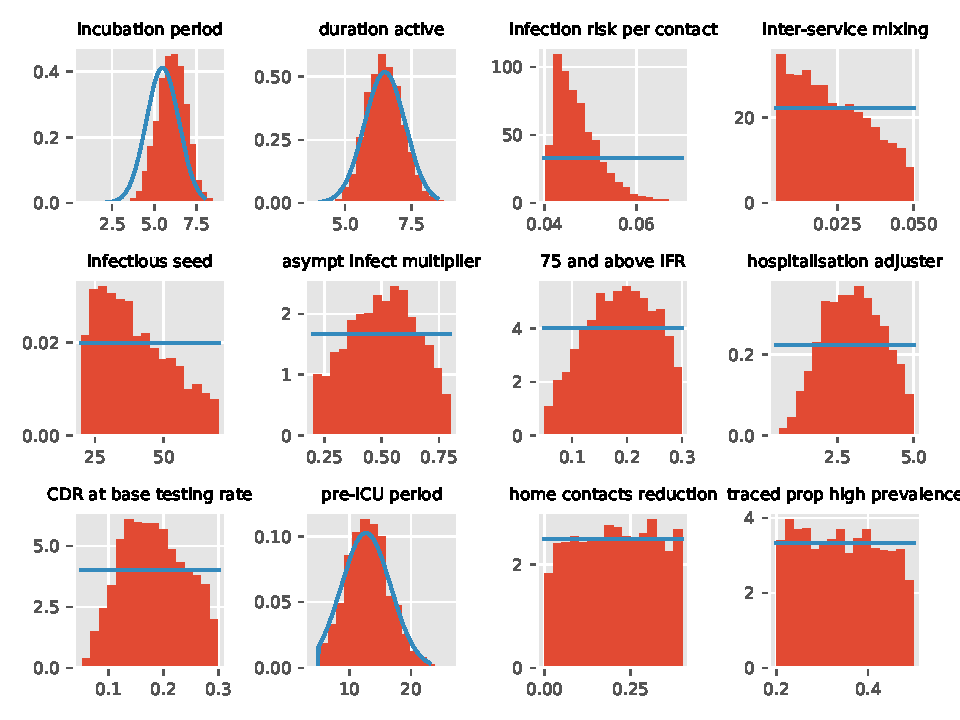
\includegraphics[scale=1]{../covid_19/projects/victoria/prem_sensitivity/epi_posteriors.png}}
    \caption{\textbf{Posterior distributions of epidemiological parameters mapping Google residential mobility to home locations of mixing matrices.}}
    \label{fig:residential_sensitivity_epi_params}
\end{figure}
